\section{Switch String}

O \textit{Switch with String} veio no Java 7 e trouxe este recurso que porém pequeno é efetivamente útil porque ajuda a escrever o código mas legível e além do mais o compilador 
irá gerar o \textit{codebyte} com mais eficiência em comparação com \textit{if-then-else}. Nos projetos analisados foram somente encontrados 77 ocorrências do \textit{switch with string}   
\begin{figure}[h]
	\center
	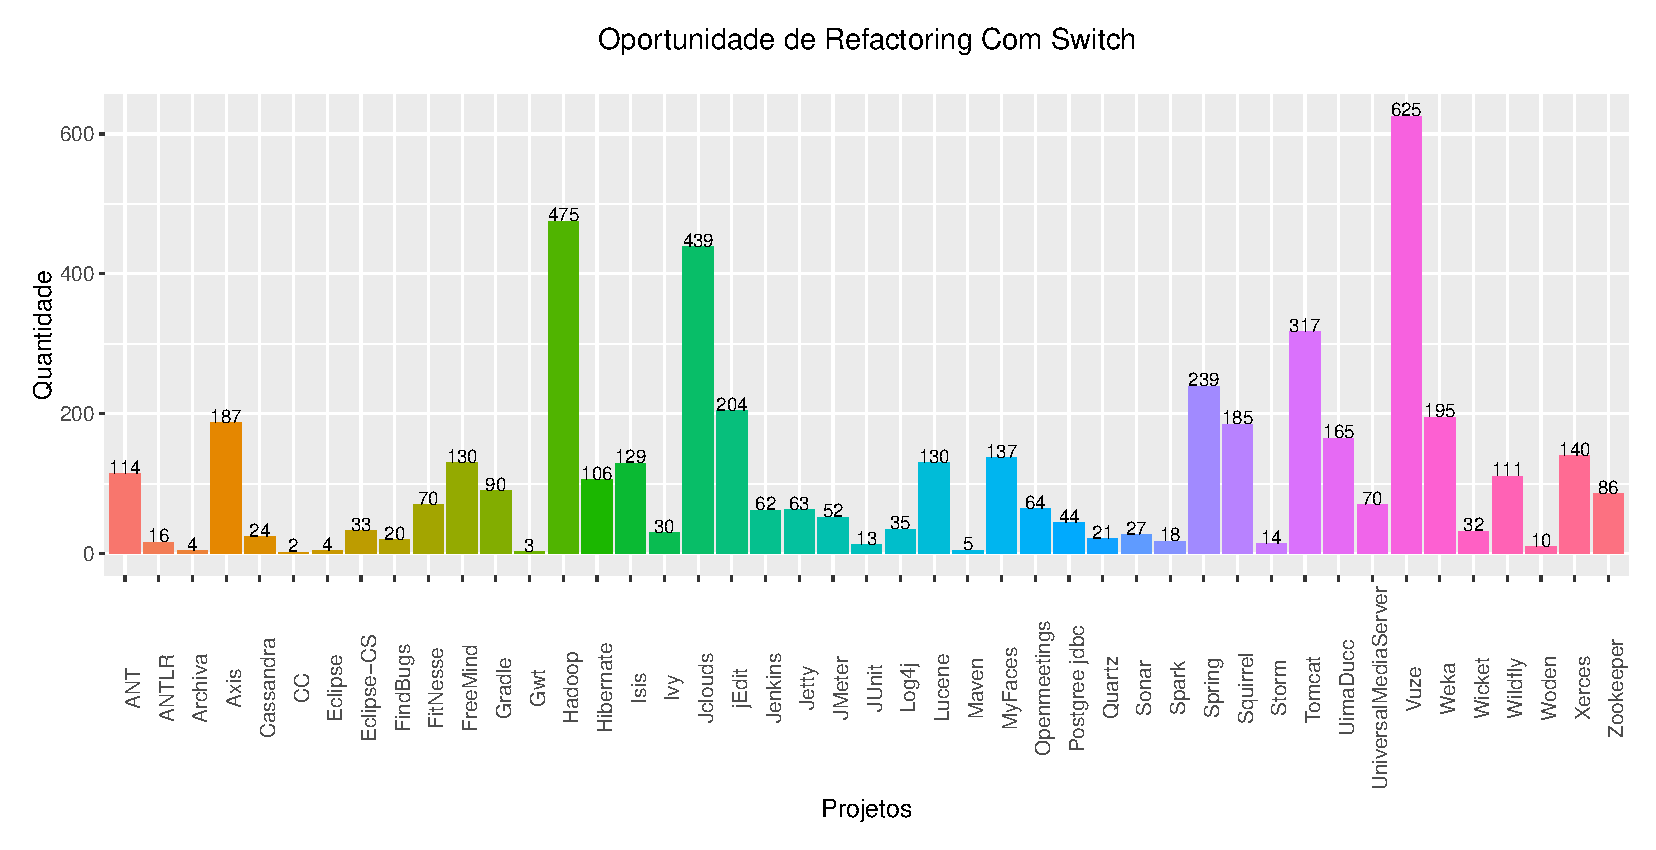
\includegraphics[scale=0.5]{Imagens/oportunidadesSwitchString}
	\label{fig:Switch with String}
	\caption{Oportunidades de \textit{Switch with String} nos projetos.}
\end{figure}

Como visto na imagem acima das diferentemente do \textit{switch with string} o uso desse recurso é mais disseminado entre os projetos analisados mas como mostra o gráfico mas de 40\% do total dos \textit{switch} do projeto \textit{Weka} pode ser transformado em \textit{switch with string} e o projeto \textit{Checkstyle} a redução é de 21\%. 

\clearpage